\documentclass[
   %handout
 ]{beamer}
 
\usetheme{simple}
\usepackage{lmodern}
\usepackage[scale=2]{ccicons}

%Codifica dei font di input e di output
\usepackage[T1]{fontenc}
\usepackage[utf8]{inputenc}

% Converte file eps in pdf
\usepackage{epstopdf}

% Consente di rappresentare i simboli di check e di cross
\usepackage{pifont}

% Consente di suddividere una colonna in due righe
\usepackage{multirow}

% Consente di rappresentare la funzione identità
\usepackage{dsfont}

% Consente di impostare le virgolette del discorso diretto
\usepackage{dirtytalk}

% Consente di impostare i commenti multiline
\usepackage{verbatim}

% Consente di disegnare grafi
\usepackage{tikz}

% Libreria per disegnare cerchi e frecce di tikz
\usetikzlibrary{arrows}

% Definizione della cartella contenente le immagini da usare
\graphicspath{{img/}}

% Disabilitare la trasparenza sulla pause
\setbeamercovered{invisible}

            
% TODO
% Finire Parte algoritmo di apprendimento
% Backpropagation
% Migliorare la spiegazione delle slide


% Watermark background (simple theme)
%\setwatermark{\includegraphics[height=8cm]{img/Heckert_GNU_white.png}}
     
%\institute{\url{http://github.com/famuvie}}

% Metadati di apertura del pdf
\hypersetup{
    pdftoolbar=true,        % show Acrobat’s toolbar?
    pdfmenubar=true,        % show Acrobat’s menu?
    pdffitwindow=false,     % window fit to page when opened
    pdfstartview={FitH},    % fits the width of the page to the window
    pdfencoding=auto
}

% Definizione degli autori
\author {
            \hspace*{0.01em}{\Large Michele Valsesia}
            %\texorpdfstring{\hspace*{0.01em}{\Large Michele Valsesia}}{Michele Valsesia} 
            %\texorpdfstring{\\ \bigskip}{e}
            %\texorpdfstring{\hspace*{0.3em}{\Large Nicholas Aspes }}{Nicholas Aspes}
        }

\begin{document}

% Definizione del Titolo e Anno Accademico

\title{Implementazione di una \\ 
       Rete Convoluzionale in CUDA \bigskip}
        
\date{\Large Anno accademico 2018/2019}


% Titolo della Presentazione
     
\begin{frame}
\maketitle
\end{frame}

% //////////////////////////////// Introduzione ////////////////////////////////////////


\begin{frame}{Introduzione}
    \framesubtitle{Obiettivi}  
    
    \begin{itemize} [<+->]
        \setlength\itemsep{3em}
        \item \large Descrivere l'architettura ed il funzionamento di una \emph{Rete Neurale Semplice} e di una \emph{Convoluzionale}
        \item \large Motivare le differenti scelte implementative adottate durante lo svolgimento del progetto
        \item \large Valutare l'accuratezza e lo speedup della rete rispetto ad una implementazione di tipo sequenziale       
    \end{itemize}  
\end{frame}


% //////////////////////////////// Parte Teorica Reti Neurali //////////////////////////

\begin{frame}[c]
  \centering
  \bigskip \bigskip    
  \Huge Reti Neurali
\end{frame}

\begin{frame}{Reti Neurali}
    \framesubtitle{Scopo}
    \begin{itemize} [<+->]
        \setlength\itemsep{2em}
        \item \large Le \emph{Reti Neurali} vengono principalmente usate per la classificazione di immagini
       \item \large Il processo di classificazione consiste nell'assegnare ad un immagine un'etichetta che identifichi nel miglior modo possibile il suo contenuto semantico
       \item \large Un'etichetta è meglio conosciuta con il nome di \emph{classe}
       \item \large Le reti neurali ricevono in input un'immagine e restituiscono in output la relativa classe 
    \end{itemize}
\end{frame} 

\begin{frame}{Reti Neurali}
    \framesubtitle{Funzionamento}
    \begin{itemize} [<+->]
        \setlength\itemsep{1em}
        \item \large Una rete neurale deve \emph{apprendere} come assegnare correttamente alle immagini le varie classi
        \item \large Un \emph{esempio} è una coppia (immagine, etichetta)
        \item \large Un esempio viene creato da un team di persone che valuta il contenuto semantico di un immagine e le associa l'etichetta più adatta 
        \item \large Il \emph{training set} ed il \emph{test set} sono insiemi di esempi
        \item \large Il training set viene usato per l'addestramento (training) della rete
        \item \large Il test set serve a controllare che la rete abbia imparato a discriminare correttamente le immagini       
    \end{itemize}
\end{frame}

\begin{frame}{Reti Neurali}
    \framesubtitle{Training}
    \begin{itemize} [<+->]
        \setlength\itemsep{2em}
        \item \large Per ognuno degli esempi del training set
        
        \bigskip
        \bigskip
        
        \setbeamertemplate{itemize items}[square] 
        \begin{itemize} 
        \setlength\itemsep{3em}
            \item \large La rete assegna all'immagine corrente la classe che meglio rappresenta il suo contenuto semantico
            \item \large Se la classe di output è diversa dall'etichetta dell'esempio, la rete corregge i suoi parametri interni e passa all'immagine successiva
        \end{itemize}
    \end{itemize}
\end{frame}

\begin{frame}{Reti Neurali}
    \framesubtitle{Testing}
    \begin{itemize} [<+->]
        \setlength\itemsep{2em}
        \item \large L'\emph{accuratezza} della rete è data dal rapporto tra il numero di esempi classificati correttamente e la cardinalità del test set
        
        \item \large Per ognuno degli esempi del test set
        
        \bigskip
        
        \setbeamertemplate{itemize items}[square] 
        \begin{itemize} 
        \setlength\itemsep{2em}
           \item \large La rete assegna all'immagine corrente la classe che meglio rappresenta il suo contenuto semantico
            \item \large Per sapere il numero di immagini classificate correttamente dalla rete è necessario definire un contatore
            \item \large Il contatore viene incrementato quando l'output prodotto è uguale all'etichetta dell'esempio considerato
        \end{itemize}
    \end{itemize}
\end{frame}

\begin{frame}{Reti Neurali}
    \framesubtitle{Significato Biologico}
    \begin{itemize} [<+->]
        \setlength\itemsep{3em}
        \item \large Le \emph{Reti Neurali} nascono con lo scopo di modellare una rete neurale biologica
       \item \large Una rete neurale biologica si compone di unità cellulari di base: i \emph{neuroni}
       \item \large I neuroni sono collegati tra loro per mezzo di specifiche giunture chiamate \emph{sinapsi}
    \end{itemize}
\end{frame} 

\begin{frame}{Reti Neurali}
    \framesubtitle{Neurone}
    
    \begin{center}
      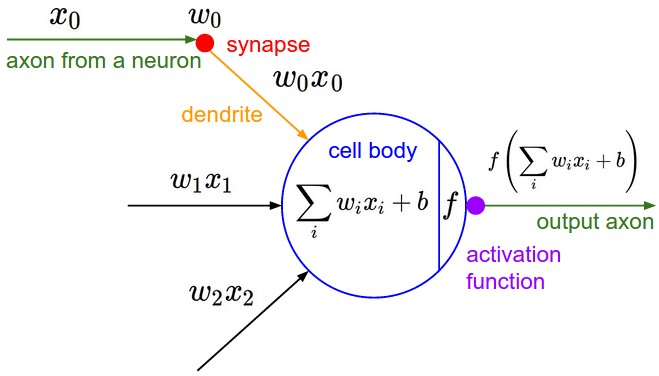
\includegraphics[scale = 0.35]{neuron_model.jpeg}
    \end{center}
  
    \bigskip 
  
  \begin{itemize}
    \setlength\itemsep{1em}
    \item[] \large \emph{Modello matematico di un neurone}
  \end{itemize}       
\end{frame} 


\begin{frame}{Reti Neurali}
    \framesubtitle{Funzionamento Neurone}
    \begin{itemize} [<+->]
        \setlength\itemsep{2em}
        \item \large Attraverso un meccanismo di eccitazione ed inibizione i pesi sinaptici controllano quanto un neurone sia influenzato dagli altri
       \item \large I segnali in ingresso al neurone vengono pesati dalle differenti sinapsi, trasportati dai dendriti all'interno del corpo cellulare e sommati tra loro
       \item \large Quando la somma supera una certa soglia, il neurone \emph{spara} un segnale lungo l'assone 
       \item \large La \emph{frequenza di sparo} del neurone viene modellata con una funzione di attivazione $f$       
    \end{itemize}
\end{frame}


\begin{frame}{Reti Neurali}
    \framesubtitle{Funzioni di Attivazione}
    \begin{block}{Definizione} 
        \large Una \emph{funzione di attivazione} è una funzione matematica non lineare usata per modellare l'output di un neurone. L'input è dato dalla somma pesata dei segnali in ingresso al neurone
    \end{block}\pause
    
    \bigskip
    
    \begin{itemize} [<+->]
        \setlength\itemsep{1.5em}
        \item \emph{\large Rectifier Linear Unit}
        \item \emph{\large Sigmoide}
        \item \emph{\large Tangente Iperbolica}
        \item \emph{\large Softplus}
    \end{itemize}
\end{frame}

\begin{frame}{Reti Neurali}
    \framesubtitle{Rectifier Linear Unit}
    \begin{block}{Definizione} 
        \large La \emph{Rectifier Linear Unit (ReLU)} $r: \mathbb{R} \rightarrow [0, +\infty)$ è definita come $r(x) = \max(0,x)$  
    \end{block}\pause
    
    \bigskip
    
    \begin{itemize} [<+->]
        \setlength\itemsep{2em}
        \item \large Si differenzia da una funzione di tipo lineare per metà del suo dominio in quanto $\forall x < 0, max(0,x) = 0$
        \item \large Presenta un punto di discontinuità in $x = 0$
        \item \large La sua derivata è pari a $r^{\prime}(x) = \mathds{1}(x \geq 0)$
    \end{itemize}
\end{frame}


\begin{frame}{Reti Neurali}
    \framesubtitle{Rectifier Linear Unit}
    
    \begin{center}
      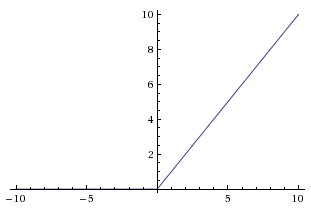
\includegraphics[scale = 0.6]{relu.jpeg}
    \end{center}
  
    \bigskip 
  
  \begin{itemize}
    \setlength\itemsep{1em}
    \item[] \large \emph{Rappresentazione grafica ReLU}
  \end{itemize}       
\end{frame} 

\begin{frame}{Reti Neurali}
    \framesubtitle{Sigmoide}
    \begin{block}{Definizione} 
        \large La \emph{Sigmoide} $\sigma: \mathbb{R} \rightarrow [0, 1]$ è definita come $\sigma(x) = \frac{1}{(1 + e^{-x})}$ 
    \end{block}\pause
    
    \bigskip
    
    \begin{itemize} [<+->]
        \setlength\itemsep{2em}
        \item \large Per elevati valori negativi di input la sigmoide restituisce 0: il neurone non spara affatto
        \item \large Per elevati valori positivi la sigmoide restituisce 1: il neurone satura e spara con frequenza di sparo pari a 1
        \item \large La sua derivata è uguale a $\sigma^{\prime}(x) = \sigma(x)(1 - \sigma(x))$
    \end{itemize}
\end{frame}

\begin{frame}{Reti Neurali}
    \framesubtitle{Sigmoide}
    
    \begin{center}
      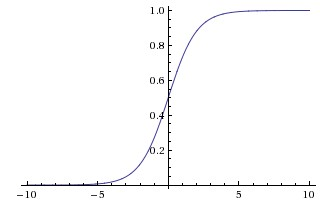
\includegraphics[scale = 0.6]{sigmoid.jpeg}
    \end{center}
  
    \bigskip 
  
  \begin{itemize}
    \setlength\itemsep{1em}
    \item[] \large \emph{Rappresentazione grafica Sigmoide}
  \end{itemize}       
\end{frame} 



\begin{frame}{Reti Neurali}
    \framesubtitle{Tangente Iperbolica}
    \begin{block}{Definizione} 
        \large La \emph{Tangente Iperbolica} $\tanh: \mathbb{R} \rightarrow [-1, 1]$ è definita come $\tanh(x) = 2\sigma(2x) - 1$ 
    \end{block}\pause
    
    \bigskip
    
    \begin{itemize} [<+->]
        \setlength\itemsep{2em}
        \item \large La tangente iperbolica è una sigmoide scalata
        \item \large A differenza della sigmoide passa dall'origine per $x = 0$ 
        \item \large La sua derivata è uguale a $\tanh^{\prime}(x) = 1 - \tanh^{2}(x)$
    \end{itemize}
\end{frame}

\begin{frame}{Reti Neurali}
    \framesubtitle{Tangente Iperbolica}
    
    \begin{center}
      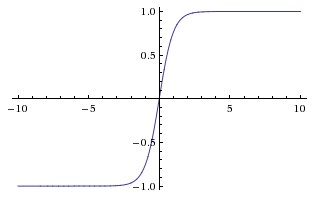
\includegraphics[scale = 0.6]{tanh.jpeg}
    \end{center}
  
    \bigskip 
  
  \begin{itemize}
    \setlength\itemsep{1em}
    \item[] \large \emph{Rappresentazione grafica Tangente Iperbolica}
  \end{itemize}       
\end{frame} 

\begin{frame}{Reti Neurali}
    \framesubtitle{Softplus}
    \begin{block}{Definizione} 
        \large La \emph{Softplus} $s: \mathbb{R} \rightarrow (0, +\infty)$ è definita come $s(x) = \log(1 + e^x)$ 
    \end{block}\pause
    
    \bigskip
    
    \begin{itemize} [<+->]
        \setlength\itemsep{2em}
        \item \large La softplus è una buona approssimazione della ReLU
        \item \large Viene solitamente usata per sostituire la ReLU perché non presenta punti di discontinuità
        \item \large La sua derivata è uguale a $s^{\prime}(x) = \frac{1}{(1 + e^{-x})} = \sigma(x)$
    \end{itemize}
\end{frame}

\begin{frame}{Reti Neurali}
    \framesubtitle{Softplus}
    
    \begin{center}
      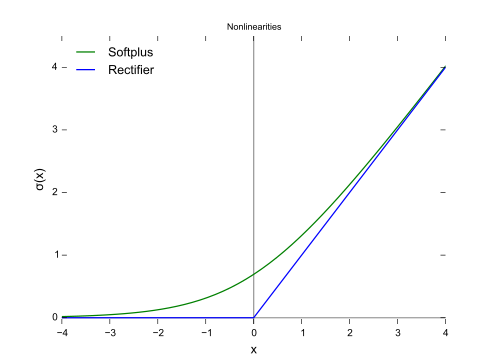
\includegraphics[scale = 0.45]{softplus_vs_rectifier.png}
    \end{center}
  
    \smallskip
  
  \begin{itemize}
    \setlength\itemsep{1em}
    \item[] \large \emph{Confronto grafico tra ReLU e Softplus}
  \end{itemize}       
\end{frame} 

\begin{frame}{Reti Neurali}
    \framesubtitle{Rete Neurale}
    
    \begin{block}{Definizione} 
        \large Una \emph{Rete Neurale} è composta da un certo numero di neuroni organizzati in insiemi distinti chiamati \emph{livelli} o \emph{layer}
    \end{block}\pause
    
    \begin{itemize} [<+->]
        \setlength\itemsep{2em}
        \item \large I livelli sono connessi tra loro e sono posizionati uno di seguito all'altro in modo da formare una sequenza
        \item \large I livelli intermedi prendono il nome di \emph{hidden}
        \item \large L'output dei neuroni di un livello diventano l'input dei neuroni del livello successivo        
    \end{itemize}
\end{frame}

\begin{frame}{Reti Neurali}
    \framesubtitle{Rete Neurale}
    
    \begin{itemize} [<+->]
        \setlength\itemsep{3em}
        \item \large Quando si effettua il conteggio dei livelli di una rete non si considera il livello di input
        \item \large Una rete a \emph{singolo livello} non presenta livelli hidden    
        \item \large Per determinare la grandezza di una rete ci si concentra sul numero di neuroni e sui relativi pesi ad essi associati
    \end{itemize}
\end{frame}

\begin{frame}{Reti Neurali}
    \framesubtitle{Livello Fully-Connected}
    
    \begin{block}{Definizione} 
        \large Un livello è di tipo \emph{Fully-Connected} quando i neuroni che lo compongono sono completamente connessi ai neuroni del livello successivo e non sono collegati tra loro internamente 
    \end{block}\pause
    
    \begin{itemize} [<+->]
        \setlength\itemsep{1.5em}
        \item \large I pesi dei neuroni di ciascun livello sono salvati all'interno di matrici
        \item \large Le righe di una matrice identificano i neuroni del livello mentre le colonne contengono i pesi di ciascun neurone
        \item \large La struttura a livelli di una rete neurale permette di sfruttare le potenzialità del calcolo matriciale 
    \end{itemize}
\end{frame}

\begin{frame}{Reti Neurali}
    \framesubtitle{Livello Fully-Connected}
    
    \begin{center}
      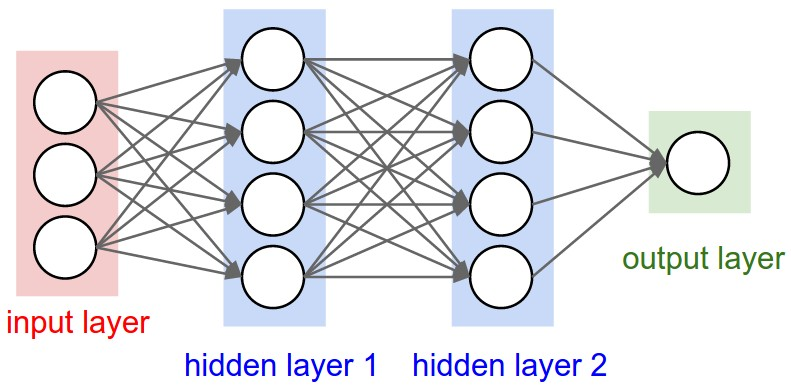
\includegraphics[scale = 0.35]{fully_connected.jpeg}
    \end{center}
  
    \bigskip
  
    \begin{itemize}
        \setlength\itemsep{1em}
        \item[] \large \emph{Una rete neurale a 3 livelli}
    \end{itemize}       
\end{frame} 



\begin{frame}{Reti Neurali}
    \framesubtitle{Funzionamento}
    
    Il processo di apprendimento di una rete neurale è suddiviso in quattro fasi distinte \pause
    
    \bigskip
    \bigskip
    
    \begin{itemize} [<+->]
        \setlength\itemsep{2em}
        \item \emph{\large Inizializzazione dei pesi}
        \item \emph{\large Forward Propagation}
        \item \emph{\large Calcolo della Funzione di Perdita}
        \item \emph{\large Back Propagation}
    \end{itemize}
\end{frame}

\begin{frame}{Reti Neurali}
    \framesubtitle{Inizializzazione dei pesi}
    
    \smallskip
    
    \begin{itemize} [<+->]
        \setlength\itemsep{3em}
        \item \large Al momento della nascita gli esseri umani non sono in grado di discriminare nessun tipo di oggetto a causa del mancato addestramento della loro rete neurale biologica
        \item \large Per riprodurre questo comportamento, all'inizio della fase di training, i pesi sinaptici $w_i$ di ciascun livello vengono inizializzati in maniera casuale     
    \end{itemize}
\end{frame}



\begin{frame}{Reti Neurali}
    \framesubtitle{Forward Propagation}
    
    \begin{block}{Definizione} 
        \large La \emph{Forward Propagation} è il meccanismo utilizzato da una rete neurale per associare ad un'immagine una determinata classe
    \end{block}\pause
    
    \smallskip
        
    \begin{itemize} [<+->]
        \setlength\itemsep{1em}
        \item \large L'output dei neuroni del livello $i$ viene moltiplicato per la matrice dei pesi del livello $i+1$ ottenendo il vettore $v$
        \item \large Al vettore $v$ viene aggiunto il vettore dei bias del livello $i+1$
        \item \large L'output del livello $i+1$ si ottiene applicando la funzione di attivazione $f$ ad ogni entry del vettore $v$
        \item \large Le operazioni precedenti sono svolte per tutti i livelli ad eccezione dell'ultimo
    \end{itemize}
\end{frame}

\begin{frame}{Reti Neurali}
    \framesubtitle{Calcolo della funzione di perdita}
    
    \begin{block}{Definizione} 
        \large Una \emph{funzione di perdita} $L$ viene utilizzata per determinare l'errore di classificazione di una rete neurale
    \end{block}\pause
        
    \begin{itemize} [<+->]
        \setlength\itemsep{1em}
        \item \large La funzione di perdita più usata è la \emph{Mean Squared Error (MSE)} $L = \frac{1}{2} \sum (y - o)^{2}$
        \item \large $y$ identifica l'etichetta dell'esempio considerato mentre $o$ l'output della rete 
        \item \large Minimizzando la funzione di perdita $L$ si riduce l'errore di una rete neurale
        \item \large Calcolando la derivata di $L$ in funzione dei pesi $w_i$ si cerca di individuare il minimo globale della funzione di perdita
    \end{itemize}
\end{frame}

\begin{frame}{Reti Neurali}
    \framesubtitle{Funzione di perdita}
    
    \begin{center}
      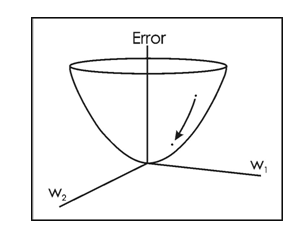
\includegraphics[scale = 0.7]{Loss.png}
    \end{center}
  
    \smallskip
  
    \begin{itemize}
        \setlength\itemsep{1em}
        \item[] \large \emph{Mean Squared Error (MSE). I pesi $w_1$ e $w_2$ sono le variabili indipendenti. La funzione di perdita $L$ è la variabile dipendente}
    \end{itemize}       
\end{frame} 

\begin{frame}{Reti Neurali}
    \framesubtitle{Back Propagation}
    
    \begin{block}{Definizione} 
        \large La \emph{Back Propagation} è il meccanismo utilizzato da una rete neurale per correggere gli errori di classificazione. Vengono individuati i pesi $w_i$ che hanno influenzato maggiormente l'errore commesso e viene aggiornato il loro valore in modo da ridurre la funzione di perdita
    \end{block}\pause
    
    \bigskip 
    
    \begin{itemize} [<+->]
        \setlength\itemsep{2em}
        \item \large Per calcolare la derivata della funzione $L$ in funzione dei pesi $w_i$ viene usata la \emph{regola della catena (chain rule)}
        \item \large Questa regola è usata per trovare la derivata di una funzione composta
    \end{itemize}      
\end{frame}

\begin{frame}{Reti Neurali}
    \framesubtitle{Aggiornamento dei Pesi e Learning Rate}
    
    \begin{itemize} [<+->]
        \setlength\itemsep{1.5em}
        \item \large Il nuovo valore del peso $w_i$ è dato dalla regola di aggiornamento  $w_i = w_i - \eta\frac{\partial L}{\partial w_i} = w_i + \Delta w_i$ con $\eta > 0$
        \item \large Il \emph{learning rate} $\eta$ è un parametro usato per controllare la velocità di aggiornamento dei pesi 
        \item \large Un learning rate alto comporta aggiornamenti rapidi, un tempo di esecuzione più basso, ma una maggiore probabilità di finire in un minimo locale
        \item \large Un learning rate basso diminuisce la probabilità di finire in un minimo locale, ma allunga notevolmente i tempi di esecuzione
    \end{itemize}      
\end{frame}

\begin{comment}
\begin{frame}{Reti Neurali}
    \framesubtitle{Esempio Learning Rate}
    
    \begin{center}
      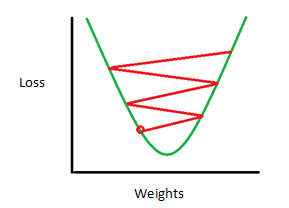
\includegraphics[scale = 0.6]{HighLR.png}
    \end{center}
    
    \bigskip
    \smallskip
    
    \begin{itemize}
        \setlength\itemsep{1em}
        \item[] \large \emph{Un learning rate $\eta$ elevato comporta ampi salti e finisce rapidamente in un minimo locale}
    \end{itemize}    
\end{frame} 

\end{comment}

\begin{frame}{Reti Neurali}
    \framesubtitle{Esempio Back Propagation}
    
    \begin{center}
      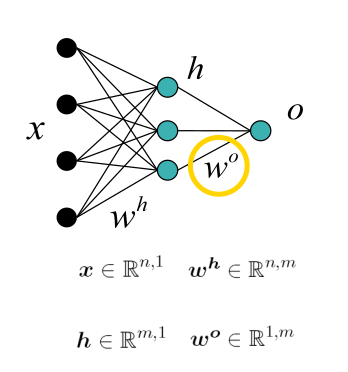
\includegraphics[scale = 0.35]{back1.png}
    \end{center}
    
    \vspace{-1em}
    
    \begin{columns}
        \begin{column}{0.48\textwidth}
            \begin{equation*}
                 \begin{split}
                    & z_j^{h} = \sum_{i=0}^{n} w_{ij}^{h}x_i \\[5pt]
                    & h_j = f(z_j^{h})
                \end{split}
            \end{equation*}            
        \end{column}
        \begin{column}{0.48\textwidth}
            \begin{equation*}
                \begin{split}
                    & z^{o} = \sum_{j=0}^{m} w_{j}^{o}h_j \\[5pt]
                    & o = f(z^{o})
                \end{split}
            \end{equation*}
        \end{column}
    \end{columns}    
    
\end{frame} 

\begin{frame}{Reti Neurali}
    \framesubtitle{Esempio Back Propagation}
    \begin{itemize} [<+->]
        \setlength\itemsep{2em}
        \item \large Derivata di $L$ in funzione del peso $w_j^{o}$ 
        
        \bigskip
        \begin{center}
         \large $ \frac{\partial L}{\partial w_j^{o}} =  \frac{\partial L}{\partial o} \cdot \frac{\partial o}{\partial z^{o}} \cdot \frac{\partial z^{o}}{\partial w_j}$         
         \end{center}
         
         \bigskip
         \setbeamertemplate{itemize items}[square]
         \begin{itemize}
            \setlength\itemsep{2.5em}
            \item \large $\frac{\partial L}{\partial o} = \frac{\partial}{\partial o} \big[ \frac{1}{2}(y - o)^{2} \big] = -(y - o)$
            \item \large $\frac{\partial o}{\partial z^{o}} = f^{\prime}(z^{o})$
            \item \large $\frac{\partial z^{o}}{\partial w_j^{o}} = h_j$ 
         \end{itemize}
    \end{itemize}
\end{frame}


\begin{frame}{Reti Neurali}
    \framesubtitle{Esempio Back Propagation}
    \begin{itemize} [<+->]
        \setlength\itemsep{3em}
        \item \large Risultato della derivata di $L$ in funzione del peso $w_j^{o}$
        \bigskip
        \begin{center}
         \large $ \frac{\partial L}{\partial w_j^{o}} =  -(y - o) \cdot f^{\prime}(z^{o}) \cdot h_j = -\delta_j^{o}h_j$         
         \end{center}
         \item \large Aggiornamento del peso $w_j^{o}$
         \bigskip
         \begin{center}
         \large $ \Delta w_j^{o} = \eta\delta_j^{o}h_j$         
         \end{center}       
    \end{itemize}
\end{frame}

\begin{frame}{Reti Neurali}
    \framesubtitle{Esempio Back Propagation}
    
    \begin{center}
      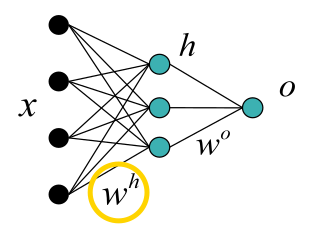
\includegraphics[scale = 0.4]{back2.png}
    \end{center}
    
    \bigskip  

     \begin{equation*}
         \frac{\partial L}{\partial w_{ij}^{h}} =  \frac{\partial L}{\partial o} \cdot \frac{\partial o}{\partial z^{o}} \cdot \frac{\partial z^{o}}{\partial h_j} \cdot \frac{\partial h_j}{\partial z_j^{h}} \cdot \frac{\partial z_j^{h}}{\partial w_{ij}^{h}}
     \end{equation*}            
\end{frame}

\begin{frame}{Reti Neurali}
    \framesubtitle{Esempio Back Propagation}
    \begin{itemize} [<+->]
        \setlength\itemsep{2em}
        
        \item[] \large \begin{center} $\frac{\partial L}{\partial o} = \frac{\partial}{\partial o} \big[ \frac{1}{2}(y - o)^{2} \big] = -(y - o)$ \end{center}
        \item[] \large \begin{center} $\frac{\partial o}{\partial z^{o}} = f^{\prime}(z^{o})$ \end{center}
        \item[] \large \begin{center} $\frac{\partial z^{o}}{\partial h_j} = w_j^{o}$ \end{center}
        \item[] \large \begin{center} $\frac{\partial h_j}{\partial z_j^{h}} = f^{\prime}(z_j^{h})$ \end{center}
        \item[] \large \begin{center} $\frac{\partial z_j^{h}}{\partial w_{ij}^{h}} = x_i$ \end{center}          
    \end{itemize}
\end{frame}


\begin{frame}{Reti Neurali}
    \framesubtitle{Esempio Back Propagation}
    \begin{itemize} [<+->]
        \setlength\itemsep{3em}
        \item \large Risultato della derivata di $L$ in funzione del peso $w_{ij}^{h}$
        \bigskip 
        \begin{center}
         \large $ \frac{\partial L}{\partial w_{ij}^{h}} =  -(y - o) \cdot f^{\prime}(z^{o}) \cdot w_j^{o} \cdot f^{\prime}(z_j^{h}) \cdot x_i = -\delta_j^{h}x_i$         
         \end{center}
         \item \large Aggiornamento del peso $w_{ij}^{h}$
         \bigskip
         \begin{center}
         \large $ \Delta w_{ij}^{h} = \eta\delta_j^{h}x_i$         
         \end{center}       
    \end{itemize}
\end{frame}

\begin{frame}{Reti Neurali}
    \framesubtitle{Rete Neurale Convoluzionale}
    
    \begin{block}{Definizione}  
    Una \emph{Rete Neurale Convoluzionale} è una variante di una rete neurale classica. Permette la condivisione dei pesi sinaptici tra i neuroni di un livello e consente di discriminare le varie feature che compongono un'immagine
    \end{block}\pause
    
    \bigskip
    
    \begin{itemize} [<+->]
        \setlength\itemsep{1em}
        \item \large Viene definito un nuovo tipo di livello: il \emph{Livello Convoluzionale}
        \item \large Un livello convoluzionale è formato da diversi \emph{filtri}
        \item \large La \emph{profondità (depth)} di un livello convoluzionale è data dal numero di filtri che lo compongono
    \end{itemize}    
\end{frame}


\begin{frame}{Reti Neurali}
    \framesubtitle{Filtri e Livelli Convoluzionali}  
    \begin{itemize} [<+->]
        \setlength\itemsep{1em}
         \item \large I filtri sono le matrici contenenti i pesi sinaptici del livello convoluzionale
        \item \large Ogni filtro ricerca all'interno delle immagini della rete una o più \emph{feature}: linee, curve, pattern
        \item \large Per apprendere nel miglior modo possibile il contenuto semantico di un'immagine, la rete deve saper ricercare feature sempre più complesse
        \item \large Mettendo in sequenza più livelli convoluzionali si possono ottenere feature complesse
        \item \large L'output di un generico livello convoluzionale $i$ diventa l'input del successivo livello $i+1$. Le feature prodotte da $i$ sono meno complesse di quelle ottenute da $i+1$
    \end{itemize}   
\end{frame}

\begin{frame}{Reti Neurali}
    \framesubtitle{Funzionamento}
    
    \begin{itemize} [<+->]
        \setlength\itemsep{3em}
        \item \large I pesi dei filtri di un livello convoluzionale sono inizializzati in maniera casuale
        \item \large Vengono utilizzate le stesse funzioni di attivazione e le stesse funzioni di perdita dei livelli fully-connected
        \item \large La forward e la back propagation sono le uniche fasi definite diversamente
    \end{itemize}
\end{frame}

\begin{frame}{Reti Neurali}
    \framesubtitle{Forward Propagation} 
    
    \begin{center}
      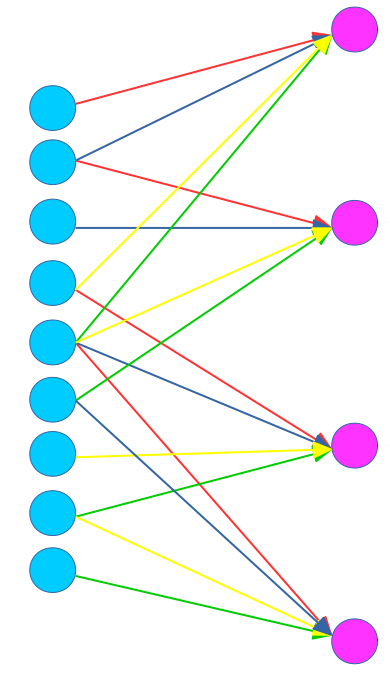
\includegraphics[scale = 0.4]{fCNN1.png}
    \end{center}
    
\end{frame}

\begin{frame}{Reti Neurali}
    \framesubtitle{Forward Propagation} 
    
    \begin{center}
      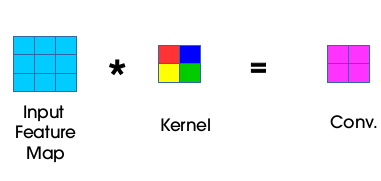
\includegraphics[scale = 0.7]{forward_conv1.png}
    \end{center}
  
    \smallskip
    
    \begin{itemize} [<+->]
        \setlength\itemsep{2em}
        \item \large Le matrici di input e di output di un livello convoluzionale prendono il nome di \emph{feature map}
        \item \large I filtri sono meglio conosciuti con il nome di \emph{kernel}
    \end{itemize}
    
\end{frame}


\begin{frame}{Reti Neurali}
    \framesubtitle{Forward Propagation} 
    
    \begin{itemize} [<+->]
        \setlength\itemsep{1em}
        \item \large All'inizio della forward propagation, il kernel viene sovrapposto alla parte superiore sinistra della feature map di input
        \item \large Viene eseguita la \emph{convoluzione} tra le due sottomatrici ed il risultato ottenuto viene salvato nella feature map di output 
        \item \large Il kernel viene spostato di una posizione verso destra e viene rieseguita nuovamente la convoluzione  
        \item \large Terminata la riga, il kernel viene posizionato nuovamente nella parte sinistra della feature map di input, ma una riga più in basso
        \item \large Gli ultimi due passaggi vengono ripetuti fino a quando non è stata riempita completamente tutta la feature map di output
    \end{itemize}
\end{frame}

\begin{frame}{Reti Neurali}
    \framesubtitle{Forward Propagation} 
    
    \bigskip
    
    \begin{center}
      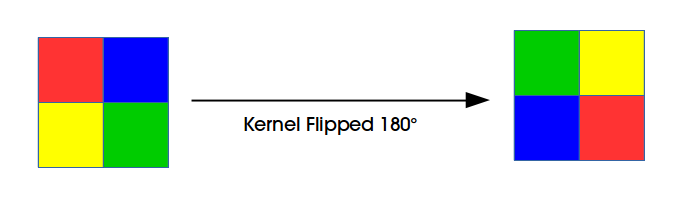
\includegraphics[scale = 0.4]{forward_flipped.png}
    \end{center}
  
    \bigskip \smallskip
        
    \begin{itemize}
        \setlength\itemsep{1em}
        \item[] \large \emph{Il kernel viene ruotato di $180^\circ$ per poter eseguire la convoluzione}
    \end{itemize}
\end{frame}

\begin{frame}{Reti Neurali}
    \framesubtitle{Forward Propagation} 
    
    \begin{center}
      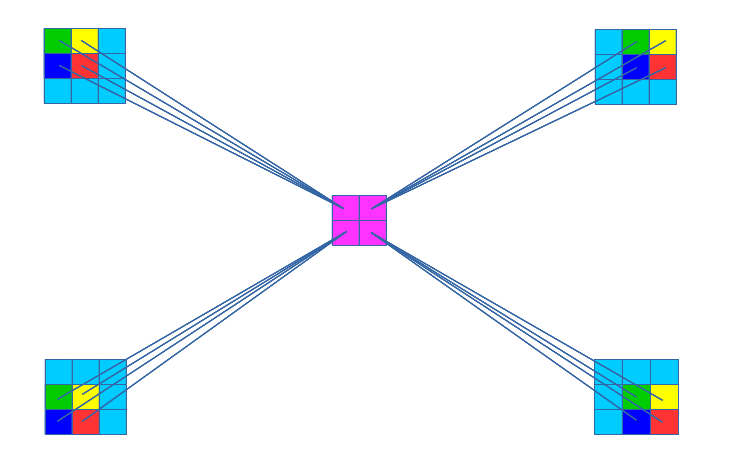
\includegraphics[scale = 0.35]{forward_conv2.png}
    \end{center}
        
    \begin{itemize}
        \setlength\itemsep{1em}
        \item[] \large \emph{Forward Propagation di un livello convoluzionale}
    \end{itemize}
\end{frame}


\begin{comment}

\begin{frame}{Reti Neurali}
    \framesubtitle{Esempio Forward Propagation} 
    
    \begin{center}
      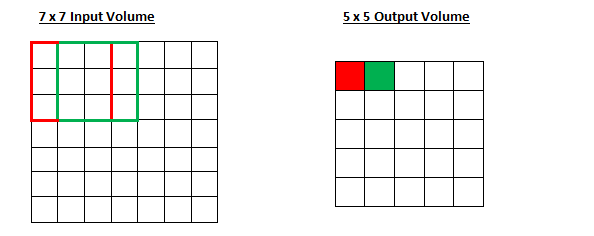
\includegraphics[scale = 0.7]{forward_conv.png}
    \end{center}
  
    \smallskip
    
    \begin{itemize}
        \setlength\itemsep{1em}
        \item[] \large \emph{Esempio di Forward Propagation. La matrice di input è un $7 \times 7$. Il filtro è un $3 \times 3$ e l'output è un $5 \times 5$}
    \end{itemize}
\end{frame}

\end{comment}

\begin{frame}{Reti Neurali}
    \framesubtitle{Considerazioni Forward Propagation} 
    
    \begin{itemize} [<+->]
        \setlength\itemsep{3em}
        \item \large Al termine della forward propagation, la funzione di attivazione $f$ viene applicata ad ogni elemento della feature map di output
        \item \large Un kernel è una matrice quadrata di dimensione $K \times K$
        \item \large La feature map di input ha dimensione $W \times H$ con $W = H$ 
        \item \large La feature map di output è una matrice quadrata di dimensione $O \times O$ con $O = (W - K) + 1$
        %\item \large La matrice di output risultante è più piccola rispetto a quella di input
        %\item \large Una sequenza di diversi livelli convoluzionali comporta la perdita di una grande quantità di informazione spaziale
        %\item \large Il \emph{padding} è il meccanismo per mezzo del quale è possibile avere una matrice di output della stessa dimensione di quella di input 
    \end{itemize}
\end{frame}

\begin{comment}
\begin{frame}{Reti Neurali}
    \framesubtitle{Padding} 
    
    \begin{itemize} [<+->]
        \setlength\itemsep{1em}
        \item \large Il padding si ottiene aggiungendo un certo numero di zeri in cima ed in fondo alle righe e alle colonne della matrice di input
        \item \large L'operazione viene fatta prima che effettuata la convoluzione con i vari filtri del livello
        \item \large Il numero di zeri da aggiungere è dato da $P = \frac{(K - 1)}{2}$
        \item \large La dimensione della matrice di output è uguale a
         \bigskip            
         \begin{center} 
             $O = (W - K + 2P) + 1$ \\
             \bigskip
             $O = (W - K + 2 \cdot \frac{(K - 1)}{2}) + 1$ \\
             \bigskip
             $O = W$ 
         \end{center}
                     
    \end{itemize}
\end{frame}
\end{comment}

\begin{frame}{Reti Neurali}
    \framesubtitle{Back Propagation}
    
    \begin{block}{Definizione}
    La Back Propagation di una rete neurale convoluzionale ha come obiettivo l'aggiornamento dei pesi contenuti nei kernel di un livello. Per ciascuno dei pesi di un kernel viene calcolata la derivata parziale $\frac{\partial L}{\partial w_{m^{\prime}, n^{\prime}}^l}$ che rappresenta l'influenza del peso $w_{m^{\prime}, n^{\prime}}^l$ sulla funzione di perdita $L$
    \end{block}\pause
    
    \bigskip
    
     \begin{itemize} [<+->]
        \setlength\itemsep{2em}
        \item \large La Back Propagation viene suddivisa in due fasi distinte
        
        \bigskip
        
        \setbeamertemplate{itemize items}[square] 
        \begin{itemize} [<+->] 
        \setlength\itemsep{1.5em}
            \item \large Il calcolo della matrice degli errori $\delta$
            \item \large L'aggiornamento dei pesi del kernel                     
        \end{itemize}
    \end{itemize}     
\end{frame}

\begin{frame}{Reti Neurali}
    \framesubtitle{Calcolo matrice dei $\delta$} 
    
    \begin{center}
      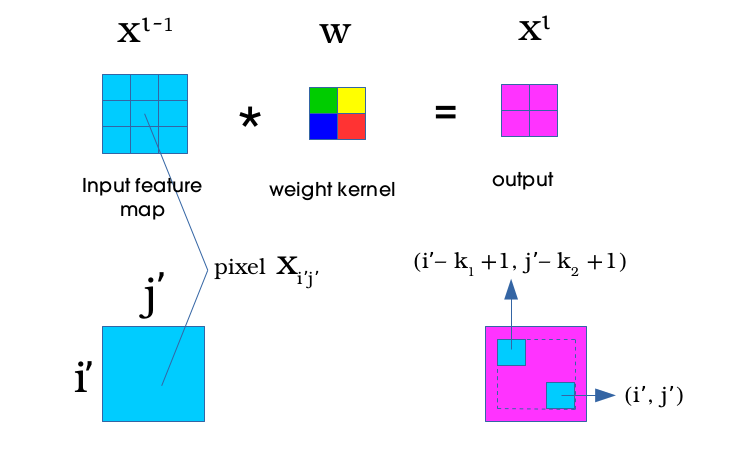
\includegraphics[scale = 0.4]{back_conv1.png}
    \end{center}
  
    \smallskip
    
    \begin{itemize}
        \setlength\itemsep{1em}
        \item[] \large \emph{Le linee tratteggiate presenti nella feature map di output individuano la regione dei pixel influenzati dal pixel $x_{i^{\prime},j^{\prime}}$. \\ $k_1$ e $k_2$ definiscono la grandezza della regione considerata}
    \end{itemize}
\end{frame}

\begin{frame}{Reti Neurali}
    \framesubtitle{Calcolo matrice dei $\delta$}
    
     \begin{itemize} [<+->]
         \setlength\itemsep{2em}
         \item \large L'influenza del pixel $x_{i^{\prime},j^{\prime}}$ sulla funzione di perdita $L$ è data da
         
         \vspace{-0.7em}
         
         \begin{align*}
         \hspace{-1cm}         
               \delta_{i^{\prime},j^{\prime}}^l = \frac{\partial L}{\partial x_{i^{\prime},j^{\prime}}^l}                 
         \end{align*}         
         
         \item \large Applicando la regola della catena si ottiene
     
    \begin{align*}        
           \frac{\partial L}{\partial x_{i^{\prime},j^{\prime}}^{l}} &= \sum_{m = 0}^{k_1 -1} \sum_{n = 0}^{k_2 -1} \frac{\partial L}{\partial x_{i^{\prime}-m, j^{\prime}-n}^{l+1}}\frac{\partial x_{i^{\prime}-m, j^{\prime}-n}^{l+1}}{\partial x_{i^{\prime},j^{\prime}}^l} \\[10pt]            
              &= \sum_{m = 0}^{k_1 -1} \sum_{n = 0}^{k_2 -1} \delta^{l+1}_{i^{\prime}-m, j^{\prime}-n} \frac{\partial x_{i^{\prime}-m, j^{\prime}-n}^{l+1}}{\partial x_{i^{\prime},j^{\prime}}^l}       
     \end{align*}    
    \end{itemize}     
\end{frame}

\begin{frame}{Reti Neurali}
    \framesubtitle{Calcolo matrice dei $\delta$}
   
     
    \begin{align*}
        \hspace{2em}          
          \frac{\partial L}{\partial x_{i^{\prime},j^{\prime}}^{l}} &= \sum_{m = 0}^{k_1 - 1} \sum_{n = 0}^{k_2 - 1} \delta^{l+1}_{i^{\prime} - m,j^{\prime} - n} w_{m,n}^{l+1} f'\left(x_{i',j'}^{l}\right) \\[10pt]
& = \text{rot}_{180^\circ} \left\{ \sum_{m = 0}^{k_1 - 1} \sum_{n = 0}^{k_2 - 1} \delta^{l+1}_{i^{\prime} + m,j^{\prime} + n} w_{m,n}^{l+1} \right\} f'\left(x_{i',j'}^{l}\right) \\[10pt]
&= \delta^{l+1}_{i',j'} \ast \text{rot}_{180^\circ} \left\{ w_{m,n}^{l+1} \right\} f'\left(x_{i',j'}^{l} \right)  
     \end{align*}        
\end{frame}

\begin{frame}{Reti Neurali}
    \framesubtitle{Aggiornamento dei pesi} 
    
    \begin{center}
      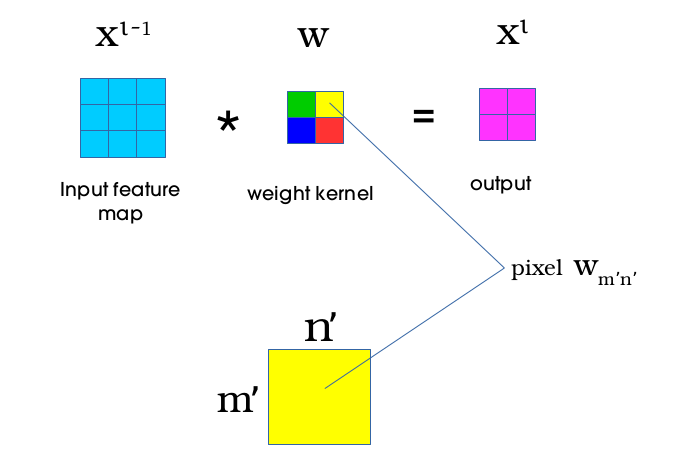
\includegraphics[scale = 0.4]{back_conv.png}
    \end{center}
  
    \smallskip
    
    \begin{itemize}
        \setlength\itemsep{1em}
        \item[] \large \emph{Durante la fase di forward propagation, il peso $w_{m^{\prime}, n^{\prime}}$ ha contribuito a calcolare tutti i valori che costituiscono la feature map di output}
    \end{itemize}
\end{frame}

\begin{frame}{Reti Neurali}
    \framesubtitle{Aggiornamento dei pesi}
     \smallskip
     \begin{itemize} [<+->]
     \setlength\itemsep{1em}
     \item \large Il calcolo di $\frac{\partial L}{\partial w_{m^{\prime}, n^{\prime}}^l}$ usando la regola della catena è dato da
     
    \begin{equation*}
        \begin{split}
            \frac{\partial L}{\partial w_{m^{\prime}, n^{\prime}}^l} & = \sum_{i=0}^{W-K} \sum_{j=0}^{W-K} \frac{\partial L}{\partial x_{i,j}^{l}} \frac{\partial x_{i,j}^{l}}{\partial w_{m^{\prime},n^{\prime}}^l} \\[10pt]
           & = \sum_{i = 0}^{W - K}\sum_{j = 0}^{W - K} \delta_{i,j}^l \cdot o_{i + m^{\prime},j + n^{\prime}}^{l-1} \\[10pt]            
           & = rot_{180^\circ} \{ \delta_{i,j}^l \} * o_{m^{\prime},n^{\prime}}^{l-1} 
        \end{split}          
    \end{equation*} 
    
    \bigskip
    
    \item \large $x_{i,j}^l = \sum_{m} \sum_{n} w_{m,n}^{l}o_{i+m, j+n}^{l-1} + b^l$         
    \item \large $o_{m^{\prime},n^{\prime}}^{l-1} = f(x_{i^{\prime},j^{\prime}}^{l-1})$    
    \end{itemize}     
\end{frame}

\begin{frame}{Reti Neurali}
    \framesubtitle{Aggiornamento dei pesi}
    
    \bigskip
    
     \begin{itemize} [<+->]
     \setlength\itemsep{3em}
    \item \large Il risultato della convoluzione tra $\delta_{i,j}^l$ e $o_{m^{\prime},n^{\prime}}^{l-1}$ individua il nuovo valore del peso $w_{m^{\prime}, n^{\prime}}^l$
    \item \large La convoluzione è svolta per ciascuno dei pesi che costituiscono un kernel     
    \end{itemize}     
\end{frame}

\begin{frame}{Reti Neurali}
    \framesubtitle{Back Propagation} 
    
    \bigskip
    
    \begin{center}
      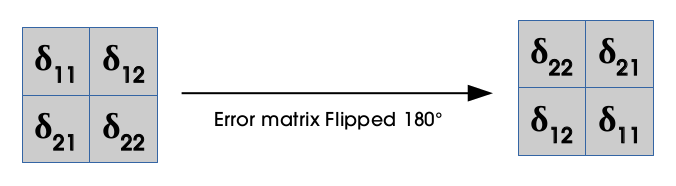
\includegraphics[scale = 0.6]{back_flipped.png}
    \end{center}
  
    \bigskip \smallskip
        
    \begin{itemize}
        \setlength\itemsep{1em}
        \item[] \large \emph{La matrice degli errori $\delta$ deve essere ruotata di $180^\circ$ per poter eseguire la convoluzione}
    \end{itemize}
\end{frame}

\begin{frame}{Reti Neurali}
    \framesubtitle{Esempio Back Propagation} 
    
    \begin{center}
      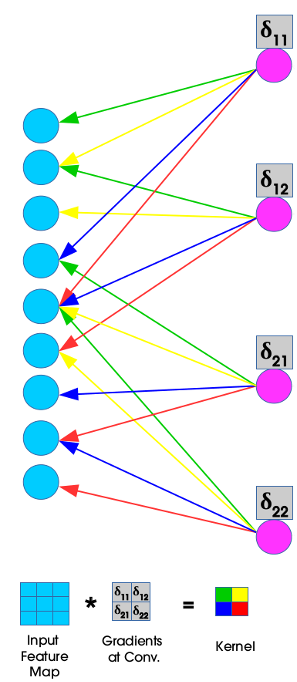
\includegraphics[scale = 0.4]{back_conv4.png}
    \end{center}
\end{frame}

\begin{frame}{Reti Neurali}
    \framesubtitle{Esempio Back Propagation} 
    
    \begin{center}
      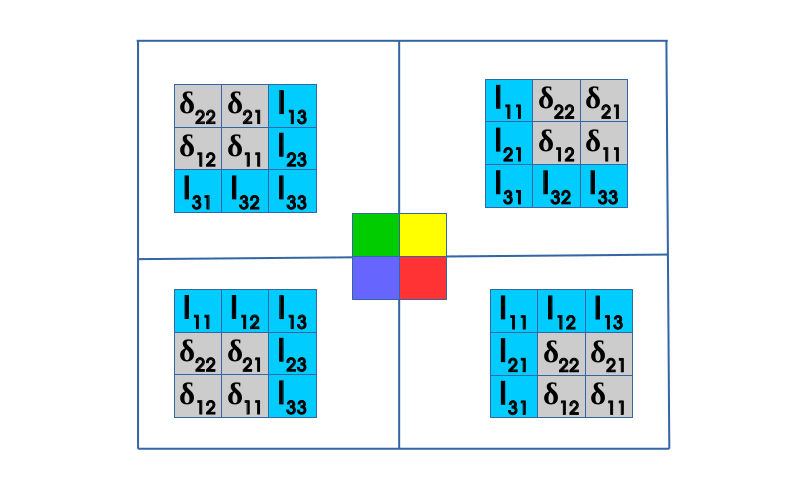
\includegraphics[scale = 0.4]{back_conv3.png}
    \end{center}
        
    \begin{itemize}
        \setlength\itemsep{1em}
        \item[] \large \emph{Il kernel aggiornato viene ricavato dalla convoluzione tra la matrice degli errori $\delta$ e la feature map di input}
    \end{itemize}
\end{frame}   

\begin{frame}[c]
  \centering
  \bigskip \bigskip    
  \Huge Implementazione della Rete
\end{frame}

\begin{frame}{Implementazione della Rete}
    \framesubtitle{Obiettivo}
    \begin{itemize} [<+->]
        \setlength\itemsep{2em}
        \item \large Si vuole costruire una rete neurale convoluzionale che permetta il riconoscimento di cifre numeriche scritte a mano
        \item \large Le cifre da riconoscere sono salvate come immagini in scala di grigio a 8 bit. Un pixel può assumere solo i valori che sono compresi nell'intervallo $[0,255]$
        \item \large L'output della rete è dato dalle 10 cifre numeriche che si vogliono riconoscere
        \item \large La rete riceve in input un'immagine e le associa la cifra numerica corrispondente
    \end{itemize}
\end{frame}


\begin{frame}{Implementazione della Rete}
    \framesubtitle{Dati}
    \begin{itemize} [<+->]
        \setlength\itemsep{3em}
        \item \large La dimensione delle immagini che costituiscono gli esempi del training e del test set hanno una dimensione di $28 \times 28$
        \item \large Le etichette sono rappresentate da numeri interi positivi
        \item \large Il training ed il test set provengono dal database \emph{MNIST} e contengono rispettativamente $60000$ esempi di train e $10000$ di test 
    \end{itemize}
\end{frame}

\begin{frame}{Implementazione della Rete}
    \framesubtitle{Rete Sequenziale}
    \begin{itemize} [<+->]
        \setlength\itemsep{3em}
        \item \large La rete sequenziale utilizzata per il confronto dei tempi di esecuzione è chiamata \emph{EduCNN}
        \item \large Ammette sia livelli di tipo fully-connected che convoluzionali
        \item \large La funzione di attivazione scelta è la sigmoide
        \item \large La rete è stata implementata usando il linguaggio di programmazione C++  
    \end{itemize}
\end{frame}

\begin{comment}
\begin{frame}{Implementazione della Rete}
    \framesubtitle{Struttura}
    \begin{itemize} [<+->]
        \setlength\itemsep{2.5em}
        \item \large La rete neurale convoluzionale sviluppata si compone di 3 livelli
        \item \large Due livelli hidden di tipo convoluzionale ed un livello di output di tipo fully-connected
        \item \large La struttura si basa su una rete neurale convoluzionale chiamata \emph{Dnn} 
        \item \large La Dnn è scritta in linguaggio C e adotta un approccio di tipo sequenziale
    \end{itemize}
\end{frame}

\begin{frame}{Implementazione della Rete}
    \framesubtitle{Struttura}
    
    \begin{table}
        \centering
        \begin{tabular}{| c | c | c | c | c |}
           \hline
           & Input & Hidden 1 & Hidden 2 & Output \\
           \hline
           \emph{Dimensione} & $28 \times 28$ & $24 \times 24$ & $20 \times 20$ & $10 \times 1$ \\ 
           \hline         
           \emph{Numero di Nodi} & 784 & 2880 & 2000 & 10 \\
           \hline
           \emph{Profondità} & 1 & 1 & 1 & 1 \\
           \hline
           \emph{Dimensione filtro} & & 5 & 5 & \\
           \hline
        \end{tabular}
    \caption{Struttura Rete Neurale}
    \end{table} 
    
    \begin{table}
        \centering
        \begin{tabular}{| c | c | c | c | c |}
           \hline
           & Input & Hidden 1 & Hidden 2 & Output \\
           \hline
           \emph{Sigmoide} & & \checkmark & \checkmark & \checkmark \\ 
           \hline         
           \emph{Tanh} & & \checkmark & \checkmark & \checkmark \\
           \hline
           \emph{Softplus} & & \checkmark & \checkmark & \checkmark \\
           \hline          
        \end{tabular}
    \caption{Funzioni di attivazione per livello}
    \end{table} 
     
    
\end{frame}
\end{comment}


\begin{frame}{Implementazione della Rete}
    \framesubtitle{Considerazioni}
    \begin{itemize} [<+->]
        \setlength\itemsep{1.5em}
        \item \large I calcoli interni alla rete vengono svolti usando il formato di dato \emph{double} in modo da non perdere precisione numerica tra i vari passaggi
        \item \large All'inizio della fase di training i pixel delle immagini vengono riscalati nell'intervallo $[0,1]$ per poter essere compatibili con il formato di dato usato dalla rete
        \item \large Tutti i dati e le strutture necessarie al funzionamento della rete vengono allocate all'inizio dell'esecuzione e deallocate al suo termine
        \item \large Le funzioni di attivazione utilizzate dalla rete CUDA sono le stesse della rete sequenziale
    \end{itemize} 
    
\end{frame}

\begin{frame}{Implementazione della Rete}
    \framesubtitle{Configurazioni}
    \smallskip
    \begin{itemize} [<+->]
        \setlength\itemsep{2em}
        \item \large Il testing della rete viene effettuato combinando tra loro differenti tipi di livelli
        \item \large Le diverse combinazioni vengono chiamate \emph{Configurazioni}
        \item \large Per studiare il comportamento della rete vengono definite quattro configurazioni
        \item \large Il numero di nodi e di livelli di ciascuna configurazione viene scelto tenendo conto della componentistica hardware utilizzata per eseguire i test
    \end{itemize}     
\end{frame}

\begin{frame}{Implementazione della Rete}
    \framesubtitle{Configurazioni}
    
     \begin{table}
        \centering
        \begin{tabular}{| c | c |}
           \hline
           \emph{Livello} & \emph{Output} \\
           \hline
           Fully Connected & $300 \times 1$  \\ 
           \hline         
           Fully Connected & $10 \times 1$ \\
           \hline
        \end{tabular}
    \caption{Configurazione 1}
    \end{table}
    
    \bigskip
    
    \begin{table}
        \centering
        \begin{tabular}{| c | c | c |}
           \hline
           \emph{Livello} & \emph{Output} & \emph{Dimensione Filtro} \\
           \hline
           Convoluzionale & $24 \times 24$ & $5 \times 5 \times 1$   \\  
           \hline 
           Fully Connected & $10 \times 1$ & \ding{55} \\
           \hline          
        \end{tabular}
    \caption{Configurazione 2}
    \end{table}
    
    
    
\end{frame}


\begin{frame}{Implementazione della Rete}
    \framesubtitle{Configurazioni}   
    
    \begin{table}
        \centering
        \begin{tabular}{| c | c | c |}
           \hline
           \emph{Livello} & \emph{Output} & \emph{Dimensione Filtro} \\
           \hline
           Convoluzionale & $22 \times 22$ & $7 \times 7 \times 1$   \\  
           \hline
           Fully Connected & $300 \times 1$ & \ding{55} \\
           \hline 
           Fully Connected & $10 \times 1$ & \ding{55} \\
           \hline          
        \end{tabular}
    \caption{Configurazione 3}
    \end{table}
    
    \bigskip    
    
    \begin{table}
        \centering
        \begin{tabular}{| c | c | c |}
           \hline
           \emph{Livello} & \emph{Output} & \emph{Dimensione Filtro} \\
           \hline
           Convoluzionale & $26 \times 26$ & $3 \times 3 \times 1$   \\  
           \hline         
           Convoluzionale & $24 \times 24$ & $3 \times 3 \times 1$   \\
           \hline
           Fully Connected & $10 \times 1$ & \ding{55} \\
           \hline          
        \end{tabular}
    \caption{Configurazione 4}
    \end{table}     
    
\end{frame}


\begin{frame}[c]
  \centering
  \bigskip \bigskip    
  \Huge Analisi dei Risultati
\end{frame}

\begin{frame}{Analisi dei Risultati}
    \framesubtitle{Hardware}
    \smallskip
    \begin{itemize} [<+->]
        \setlength\itemsep{2em}
        \item \large Le varie configurazioni sono state eseguite su una macchina che presenta le seguenti caratteristiche tecniche       
        \bigskip
        \setbeamertemplate{itemize items}[square] 
        \begin{itemize} [<+->] 
        \setlength\itemsep{2.5em}
            \item \large Processore Intel Core i7-4510 da 2.00GHz
            \item \large RAM da 6GB
            \item \large Scheda grafica Nvidia GeForce 820M da 1GB
            \item \large Sistema operativo Ubuntu 17.04                    
        \end{itemize}        
    \end{itemize}     
\end{frame}

\begin{frame}{Analisi dei Risultati}
    \framesubtitle{Parametri}
    \smallskip
    \begin{itemize} [<+->]
        \setlength\itemsep{2.5em}
        \item \large I diversi valori del learning rate $\eta$ utilizzati per testare la rete si ottengono campionando l'intervallo $[0.001, 0.8]$ a step variabili
        \item \large Per ciascuna configurazione vengono ricavati i tempi di computazione sequenziali, paralleli ed il relativo speedup
        \item \large Le configurazioni mostrate nei risultati sono quelle che hanno ottenuto il massimo valore di accuratezza in entrambe le reti
    \end{itemize}     
\end{frame}

\begin{frame}{Analisi dei Risultati}
    \framesubtitle{Risultati}
    \bigskip
    \bigskip
        \begin{table}
            \centering
            \renewcommand\arraystretch{1.3}
            \small
            \begin{tabular}{| c | c | c | c | c | c |}
                \hline
                \emph{Configurazione} & \emph{Rete} & $\eta$ & \emph{Accuratezza} & \emph{Tempo [s]} & \emph{Speedup} \\
                \hline
                \multirow{2}{*}{1} & EduCNN & 0.56 & 97.60\% & 121 & \multirow{2}{*}{2.22} \\ \cline{2-5} 
                                   & CUDA   & 0.18 & 93.86\% & 55 & \\                               
                \hline
                \multirow{2}{*}{2} & EduCNN & 0.21 & 90.64\% & 14 & \multirow{2}{*}{1.17} \\ \cline{2-5}
                                   & CUDA   & 0.20 & 84.93\% & 12 & \\
                \hline
                \multirow{2}{*}{3} & EduCNN & 0.16 & 95.58\% & 213 & \multirow{2}{*}{3.44} \\ \cline{2-5} 
                                   & CUDA   & 0.16 & 92.65\% & 62 & \\
                \hline
                \multirow{2}{*}{4} & EduCNN & 0.18 & 90.30\% & 25 & \multirow{2}{*}{0.66} \\ \cline{2-5}
                                   & CUDA   & 0.04 & 84.05\% & 38 & \\
                \hline                
            \end{tabular}
            \caption
    {\tabular[t]{@{}l@{}}Risultati delle configurazioni che hanno ottenuto il miglior \\ valore di accuratezza per un determinato learning rate $\eta$\endtabular}          
        \end{table}    
\end{frame}

\begin{frame}{Analisi dei Risultati}
    \framesubtitle{Analisi}
    \smallskip
    \begin{itemize} [<+->]
        \setlength\itemsep{2em}
        \item \large La massima differenza tra le accuratezze delle reti è del 6\%. Questa differenza è dovuta ai diversi algoritmi utilizzati dalla GPU e dalla CPU per generare i pesi casuali iniziali. A parità di pesi iniziali e di learning rate entrambe le reti producono lo stesso livello di accuratezza
        \item \large Lo speedup è significativo nelle configurazioni 1 e 3, ma inesistente o nullo nelle altre. Con kernel e livelli fully-connected di grossa taglia si ottiene un notevole vantaggio utilizzando il parallelismo, mentre per livelli più piccoli risulta migliore un approccio di tipo sequenziale
    \end{itemize}     
\end{frame}


\begin{frame}[c]
  \centering
  \bigskip \bigskip    
  \Huge Conclusioni
\end{frame}

\begin{frame}{Conclusioni}
    \framesubtitle{Conclusioni}
    \smallskip
    \begin{itemize} [<+->]
        \setlength\itemsep{3em}
        \item \large La rete CUDA risulta una buona soluzione quando si vogliono creare reti neurali semplici e convoluzionali che necessitano di grossi livelli di tipo fully-connected o convoluzionali
        \item \large Può essere utilizzata con livelli di piccole dimensioni al posto della rete sequenziale quando è richiesto che la CPU non venga troppo caricata di processi
        \item \large Non dipende da librerie di terze parti e può essere eseguita anche sui sistemi operativi Windows ed macOS
    \end{itemize}     
\end{frame}




\end{document}
